\documentclass[12pt]{article}
\usepackage[spanish]{babel}
\usepackage{graphicx}
\usepackage{float}

\title{Síntesis de redes activas \\ Laboratorio Nº1: Amplificadores ideales lineales y no lineales}

\author{Profesor Titular: Dr. Ing. Pablo Ferreyra \\  Profesor Adjunto: Ing. César Reale \\ Alumnos: Campos Mariano, 
		Enzo Verstraete}

\begin{document}
	\maketitle
	
	\begin{abstract}
		Primer laboratorio cuyo objetivo es familiarizarse con el armado y análisis de circuitos analógicos
		lineales y no lineales. En este Trabajo Práctico debe considerar para los cálculos iniciales el 
		amplificador como ideal.
	\end{abstract}
	
	
	\section{Metodología general}	
		A. Realizar una sintética introducción teórica del tema a tratar.
		B. Analizar los circuitos propuestos, todos los cálculos analíticos y su desarrollo numérico.
		C. Simulación en SPICE .
		D. Analizar las condiciones de operación límite.
		E. Armar el circuito y hacer las mediciones en laboratorio.
		F. Finalmente comparar los valores calculados, simulados y medidos, y extraer conclusiones a
		cerca de las diferencias. Analizar las causas.
		G. Presentar un informe digital, bien redactado en LÁTEX, inicializado con la propuesta del
		problema presentado por la Cátedra, los responsables del trabajo y un análisis profesional de
		cada ítem. La redacción debe ser acorde a un informe de un futuro ingeniero.
	
	\section{Introducción al análisis}
	
	El análisis del	circuito tiene como objetivo obtener una primera aproximación del comportamiento
	del circuito de manera rápida y eficiente. Para dicho análisis se tienen en cuenta las siguientes
	consideraciones.
	
	Ganancia infinita: Al considerar una ganancia infinita, la diferencia de tensión entre las entradas inversora y no inversora se hace prácticamente cero. Esto permite aplicar el concepto de masa virtual en la entrada inversora, simplificando notablemente el análisis.
	
	Impedancia de entrada infinita: La alta impedancia de entrada implica que prácticamente no circula corriente hacia las entradas del operacional, lo que facilita la aplicación de la Ley de Kirchhoff de las Corrientes (KCL) en los nodos de entrada.
	
	Impedancia de salida nula: Al considerar una impedancia de salida nula, se asume que el operacional puede suministrar cualquier cantidad de corriente sin que su tensión de salida se vea afectada, lo que simplifica el análisis de la carga conectada a la salida.
	
	\section{Circuito I: Amplificador diferencial}
	
		En esta sección se analiza el siguiente circuito.
		\begin{figure}[h]
			\centering
			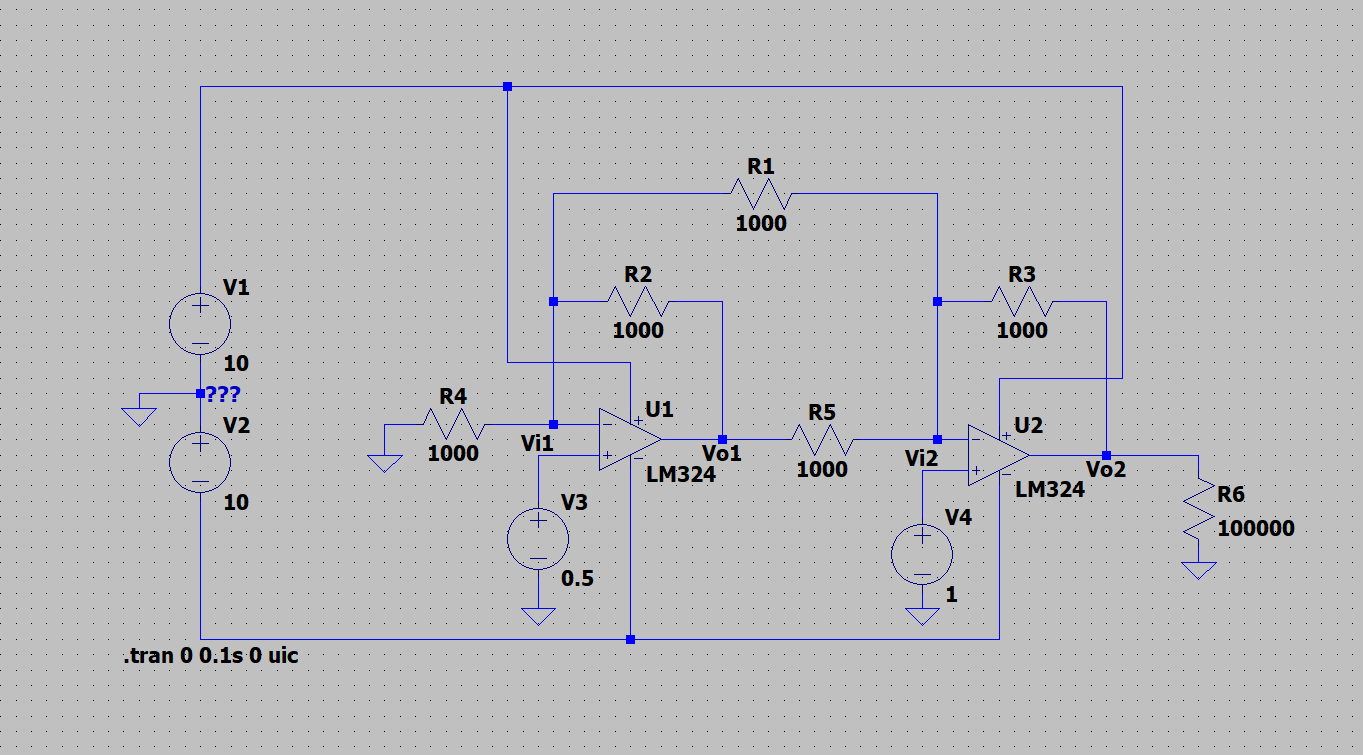
\includegraphics[width=1\linewidth]{Simulaciones-Resultados/Circuito1_esquematico}
			\caption{Amplificador diferencial}
			\label{fig:circuito1esquematico}
		\end{figure} 
		
		\subsection{Análisis del circuito}
		Para el análisis podemos hacer uso de la propiedad de superposición, considerando la salida como la suma de los
		efectos individuales de las distintas excitaciones del circuito:
		
		Análisis de $V_{01}$ por superposición de $V_1$ y $V_2$:
		
		Para $V_2=0$ queda un amplificador no inversor de $R_2$ sobre el paralelo $R_1$ y $R_4$
		\begin{equation}
			V_{01} = V_1 \,{\left(\frac{R_2 \,{\left(R_1 +R_4 \right)}}{R_1 \,R_4 }+1\right)}
		\end{equation}
		
		Normalizando los valores de la resistencia obtenemos:
		\begin{equation}
			R_1=R_2=R_3=R 
		\end{equation}
		
		La salida de $V01$ resulta:
		\begin{equation}
			V_{01}=3\,V_1
		\end{equation}
		
		Para $V_1=0$ queda un amplificador inversor de $R_2$ sobre $R_1$ 
		\begin{equation}
			V_{01} = -\frac{R_2 \,V_2 }{R_1 }
		\end{equation}
		
		Normalizando los valores de la resistencia obtenemos:
		\begin{equation}
			R_2=R_5=R 
		\end{equation}
		
		La salida de $V01$ resulta:
		\begin{equation}
			V_{01}=-V_2
		\end{equation}
		
		La salida de $V_{01}$ resulta la suma de ambos efectos, se obtiene:
		\begin{equation}
			V_{01}=3\,V_1-V_2
		\end{equation}
		
		Análisis de $V_{02}$ por superposición de $V_1$, $V_2$ y $V_{01}$:
		Para $V_1=0$ y $V_2=0$  tenemos una configuración inversora de $R_3$ sobre $R_5$
		\begin{equation}
			V_{02}=-\frac{R_3 \,V_{01} }{R_5 }
		\end{equation}
		
		Normalizando los valores de la resistencia obtenemos:
		\begin{equation}
			R_3=R_5=R 
		\end{equation}
		
		La salida de $V_{01}$ resulta:
		\begin{equation}
			V_{02}=-V_{01}
		\end{equation}
		
		Para $V_1=0$ y $V_{01}=0$ queda un amplificador no inversor de $R_3$ sobre el paralelo $R_1$ y $R_5$
		\begin{equation}
			V_{02} = V_2 \,{\left(\frac{R_3 \,{\left(R_1 +R_5 \right)}}{R_1 \,R_5 }+1\right)}
		\end{equation}
		
		Normalizando los valores de la resistencia obtenemos:
		\begin{equation}
			R_1=R_3=R_5=R 
		\end{equation}
		
		La salida de $V_{02}$ resulta:
		\begin{equation}
			V_{02}=3\,V_2
		\end{equation}
		
		Para $V_2=0$ y $V_{01}=0$  tenemos una configuración inversora de $R_3$ sobre $R_4$
		\begin{equation}
			V_{02}=-\frac{R_3 \,V_1 }{R_4 }
		\end{equation}
		
		Normalizando los valores de la resistencia obtenemos:
		\begin{equation}
			R_3=R_4=R 
		\end{equation}
		
		La salida de $V_{02}$ resulta:
		\begin{equation}
			V_{02}=-V_1
		\end{equation}
		
		La salida de $V_{02}$ resulta la suma de los tres efectos, se obtiene:
		\begin{equation}
			V_{02}=3\,V_2-V_1-V_{01}
		\end{equation}
		
		Reemplazando (7) en la ecuación anterior, se obtiene la respuesta total del circuito
		\begin{equation}
			V_{02}=4\,(V_2-V_1)
		\end{equation}
		
		\subsection{Simulación en SPICE}
		Se realizaron las simulaciones para comprobar la formula (18), se le coloca una tensión en modo común
		la tensión de salida resulta 0 como se espera.
		
		\begin{figure}[h]
			\centering
			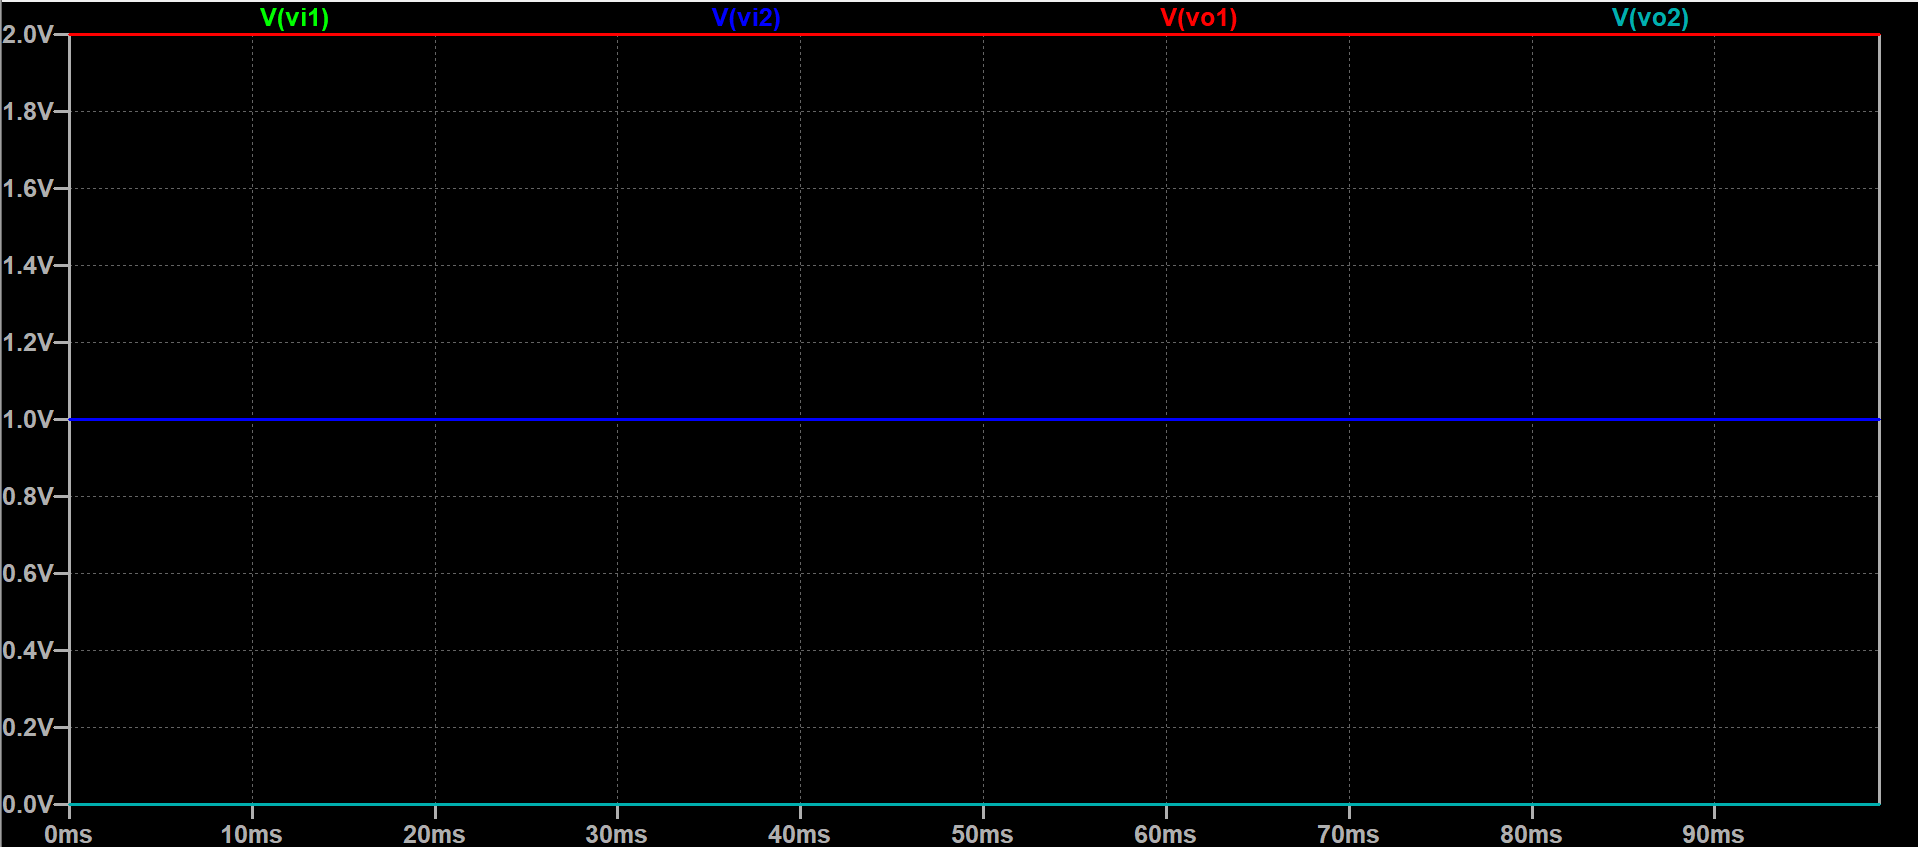
\includegraphics[width=1\linewidth]{Simulaciones-Resultados/Circuito1_Vo1(Vc)-Vo2(Vc)}
			\caption{Tensión en modo común $V_{02}=4\,(1V-1V)$}
			\label{fig:circuito1vo1vc-vo2vc}
		\end{figure} 
		
		Para tensiones diferentes la salida responde a la ecuación (18) obteniéndose los $2V$ esperados. 
		
		\begin{figure}[h]
			\centering
			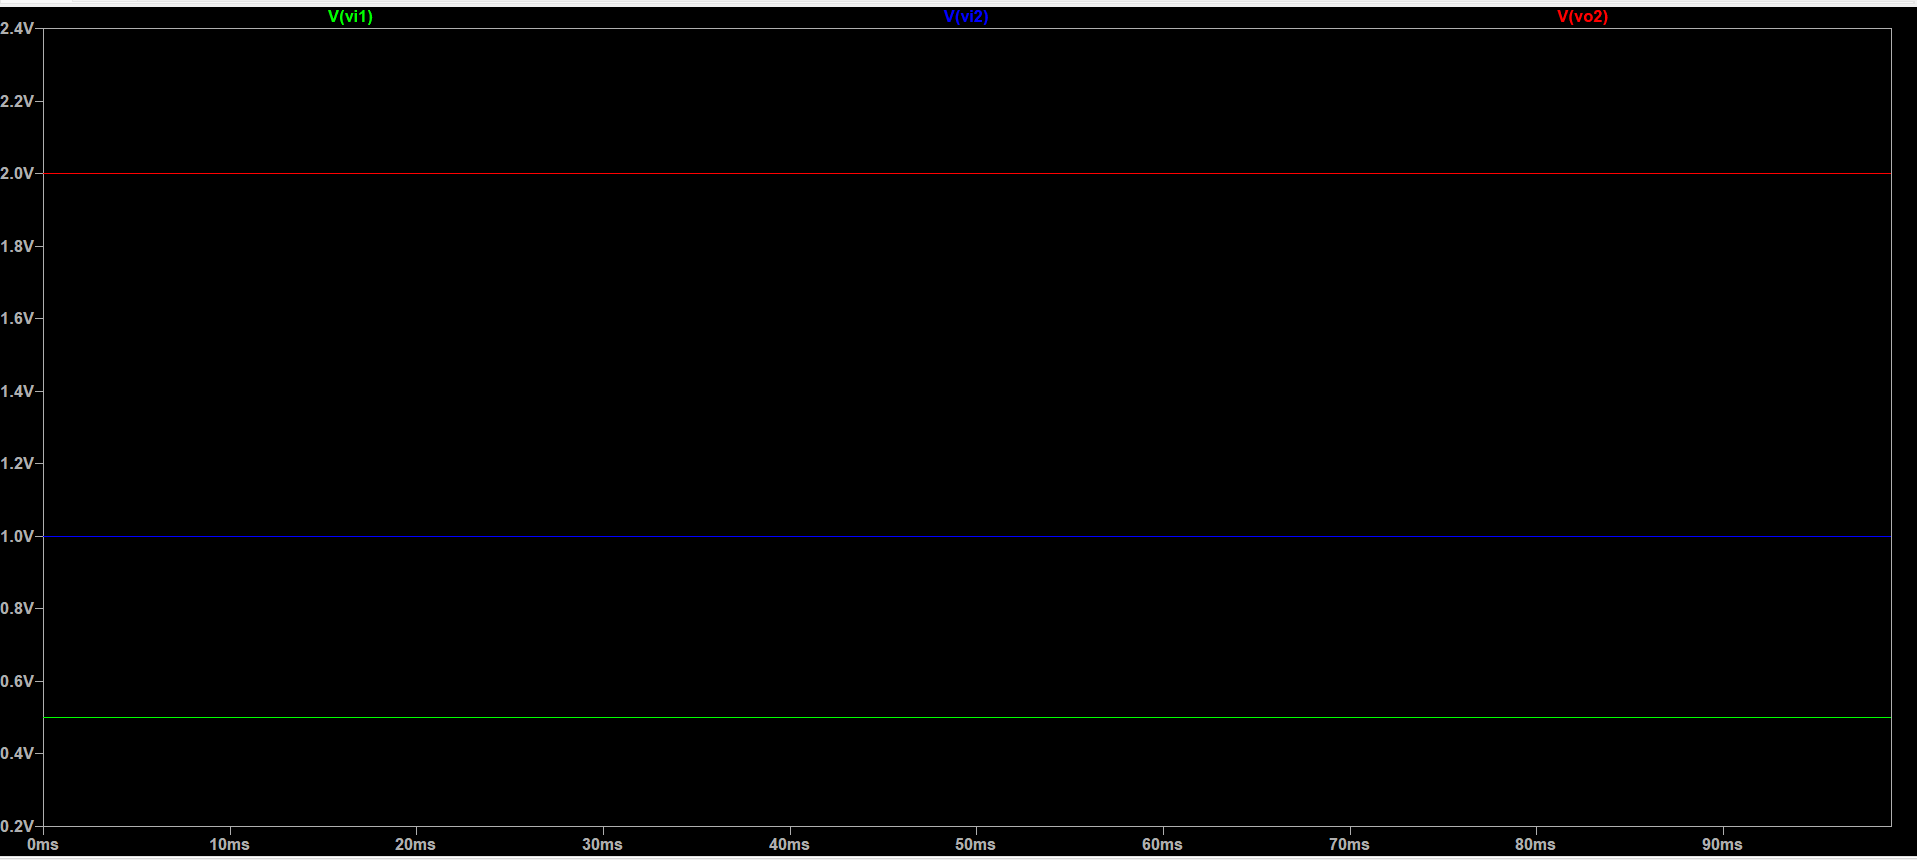
\includegraphics[width=1\linewidth]{Simulaciones-Resultados/Circuito1_Vo2-Vi1-Vi2}
			\caption{Tensiones diferentes $V_{02}=4\,(1V-0.5V)$}
			\label{fig:circuito1vo2-vi1-vi2}
		\end{figure}
			
	\section {Circuito II: Fuente de corriente controlada por tensión}
		En esta sección se analiza el siguiente circuito (Figura 4),este tipo de circuito, como su nombre indica, es un dispositivo electrónico que suministra una corriente eléctrica a una carga, pero la magnitud de esta corriente es directamente proporcional a una tensión de entrada. En otras palabras, al variar la tensión de entrada (Vin), variamos la corriente de salida (IL) de manera controlada.
		
		\begin{figure}[h]
			\centering
			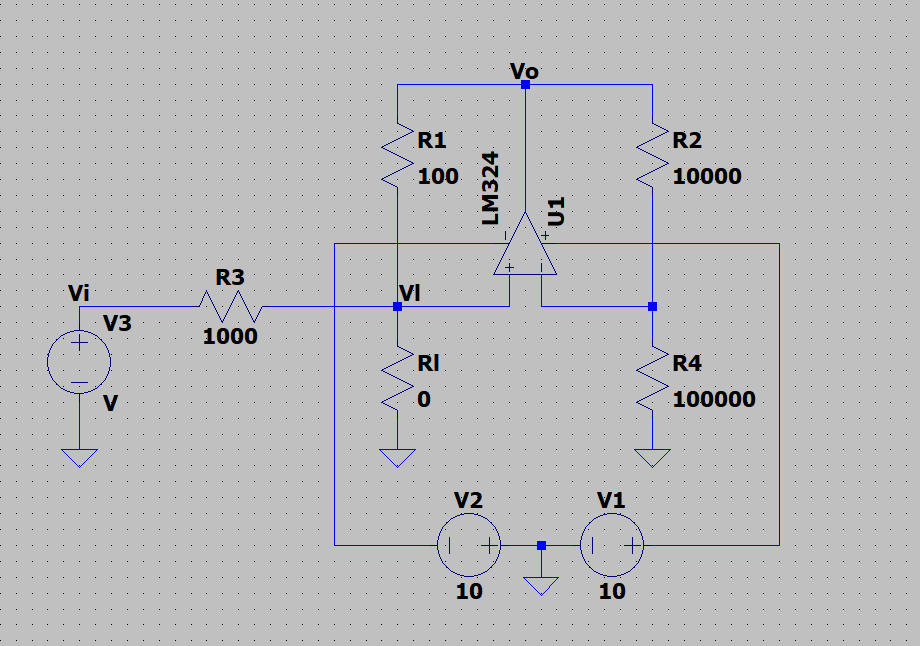
\includegraphics[width=1\linewidth]{Simulaciones-Resultados/Circuito2_esquematico}
			\caption{Fuente de corriente controlada por tensión}
			\label{fig:circuito2esquematico}
		\end{figure}
		\subsection{Análisis del circuito}
		Aplicamos ley de Kirchhoff en el nodo inversor tenemos:
		
		\begin{equation}
			-\frac{\mathrm{V_{OUT}}-\mathrm{V^-}}{R_2 }=\frac{\mathrm{V_{IN}}-\mathrm{V^-}}{R_3 }
		\end{equation}
		
		Suponiendo el amplificador ideal la tensión diferencial tiende a cero ${V^-}=0$ y despejando 
		la tensión de salida
		
		\begin{equation}
			{V_{OUT}}=-\frac{R_2 \,\mathrm{V_{IN}}}{R_3 }
		\end{equation}
		
		Obtenemos la corriente de carga con la expresión: $I_{RL}=V_{OUT}/R2$ y reemplazando en la expresión
		(20) obtenemos la corriente de carga en función del la tensión de entrada, la cual es independiente
		de R2
		
		\begin{equation}
			{I_{RL}}=-\frac{\mathrm{V_{IN}}}{R_3 }
		\end{equation} 
		
		En la siguiente tabla de valores indica las corrientes obtenidas en LTSPICE para distintos
		valores de tensión de entrada y resistencia de carga:
		\begin{table}[!ht]
			\centering
			\begin{tabular}{|l|l|l|l|l|}
				\hline
				~ & ~ & Vin[V] & ~ & ~ \\ \hline
				Irl & ~ & 0.5 & 1 & 2 \\ \hline
				Rl[Ω] & 0 & 0 & 0 & 0 \\ \hline
				~ & 1k & 495.9uA & -1.004mA & 1.996mA \\ \hline
				~ & 2k & 495.9uA & -1.0039mA & 1.996mA \\ \hline
				~ & 5k & 496.08uA & -1.004mA & 1.50mA \\ \hline
				~ & 10k & 496.3uA & -814.82uA & 763.61uA \\ \hline
			\end{tabular}
		\end{table}
	Con las simulaciones podemos ver que cuando el producto de la corriente de referencia por la resistencia supera la tensión de entrada disminuye la corriente de referencia.
		
		
	\section{Circuito III: Rectificador de precisión}
	En esta sección se analiza el siguiente circuito:
	\begin{figure}[h]
		\centering
		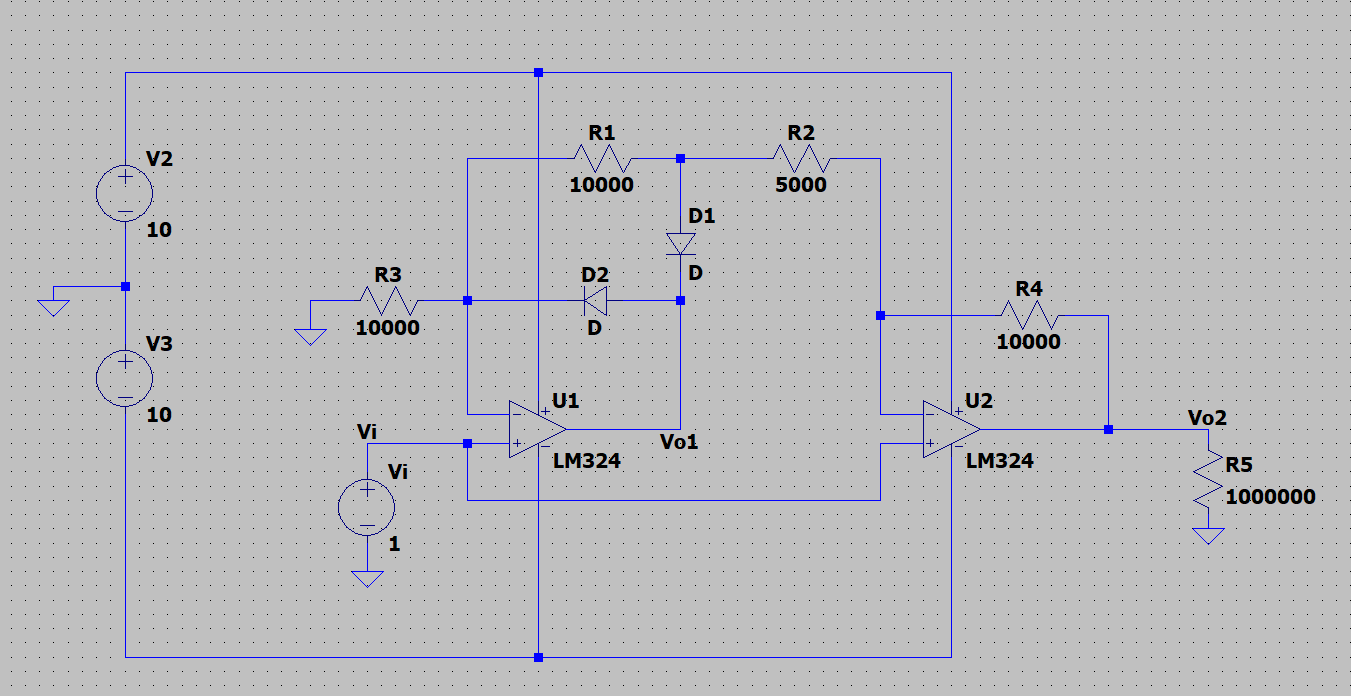
\includegraphics[width=1\linewidth]{Simulaciones-Resultados/Circuito3_esquematico}
		\caption{Rectificador de precisión}
		\label{fig:circuito3esquematico}
	\end{figure}
	El circuito que has presentado es un rectificador de precisión utilizando amplificadores operacionales. Este tipo de circuitos son muy comunes en electrónica analógica y se utilizan para convertir señales de CA a señales de CC unidireccionales, pero con una precisión mucho mayor que los rectificadores de diodo tradicionales.
		
	Hacemos un primer análisis para $V_{IN}>0$, por lo que el diodo $D_1$
	esta polarizado inversamente (circuito abierto) y $D2$ en forma directa(circuito cerrado).Obtenemos la expresión $V_{01}=f(V_{IN})$.Para este caso $Rf=0$, por lo tanto el primer operacional queda como un seguidor de tensión.
	\begin{equation}
		V_{01}=V_{IN}
	\end{equation}
	
	Obtenemos la expresión  $V_{02}=f(V_{IN})$.Para este caso resulta un amplificador no inversor.
	\begin{equation}
		V_{02}=V_{IN}1(\frac{-R4}{R1+R2})+(1+\frac{R4}{R2+R1})V_{IN}=\frac{-2}{3}V_{IN}+\frac{5}{3}V_{IN}=V_{IN}
	\end{equation}
	
		
	Para un segundo análisis proponemos que la tensión de entrada es $V_{IN}<0$ por lo tanto $D_1$ esta polarizado en directa(circuito cerrado) y $D_2$ en forma inversa (circuito abierto). Obtenemos la expresión $V_{01}=f(V_{IN})$, resulta un amplificador no inversor:
	\begin{equation}
		V_{01}=(1+\frac{R1}{R3})V_{IN}=2V_{IN}
	\end{equation}
	
	Obtenemos la expresión  $V_{02}=f(V_{IN})$.Para este caso resulta un amplificador no inversor.
	\begin{equation}
		V_{02}=(1+\frac{R1}{R3})V_{IN}\frac{-R4}{R2}+(1+\frac{R4}{R2})V_{IN}=-4V_{IN}+3V_{IN}=-V_{IN}
	\end{equation}
	
	\begin{figure}[h!]
		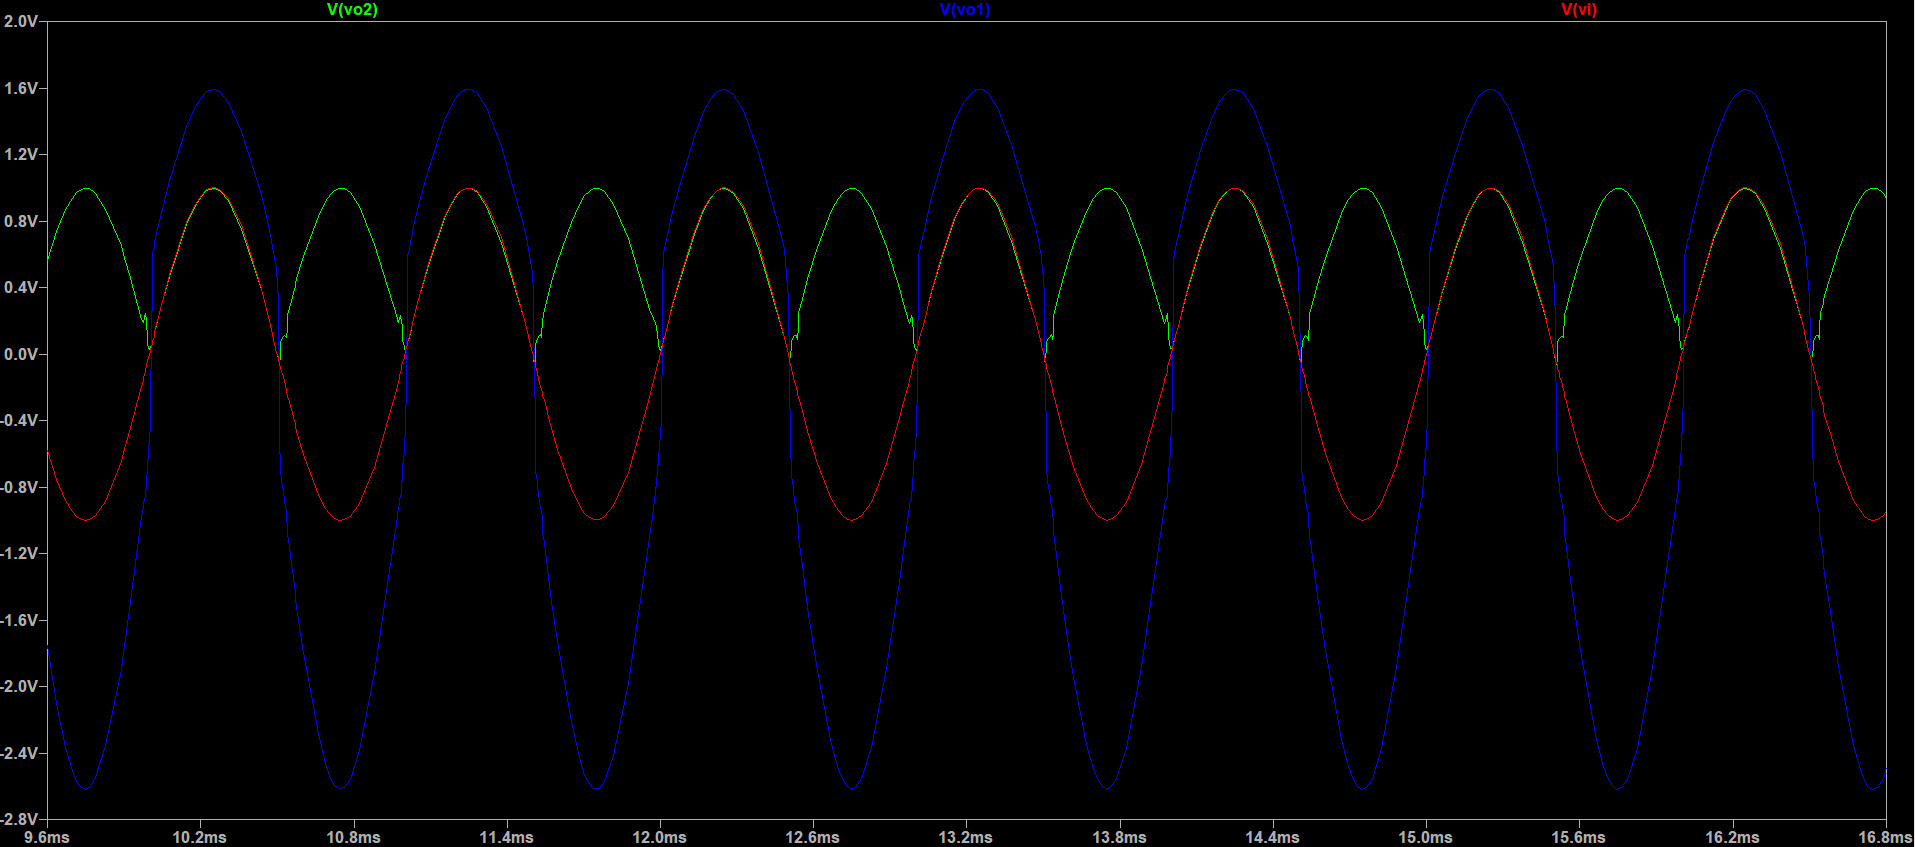
\includegraphics[width=\linewidth]{Simulaciones-Resultados/Circuito3_Vo1(Vin)-Vo2(Vin)}
		\caption[Salida de la onda rectificada]{Salida de la onda rectificada}
		\label{fig:circuito3vo1vin-vo2vin}
	\end{figure}
	
	\section{Circuito IV: Comparador con histéresis}
	Ahora, pasaremos a analizar el siguiente circuito:
	\begin{figure}[h!]
		\centering
		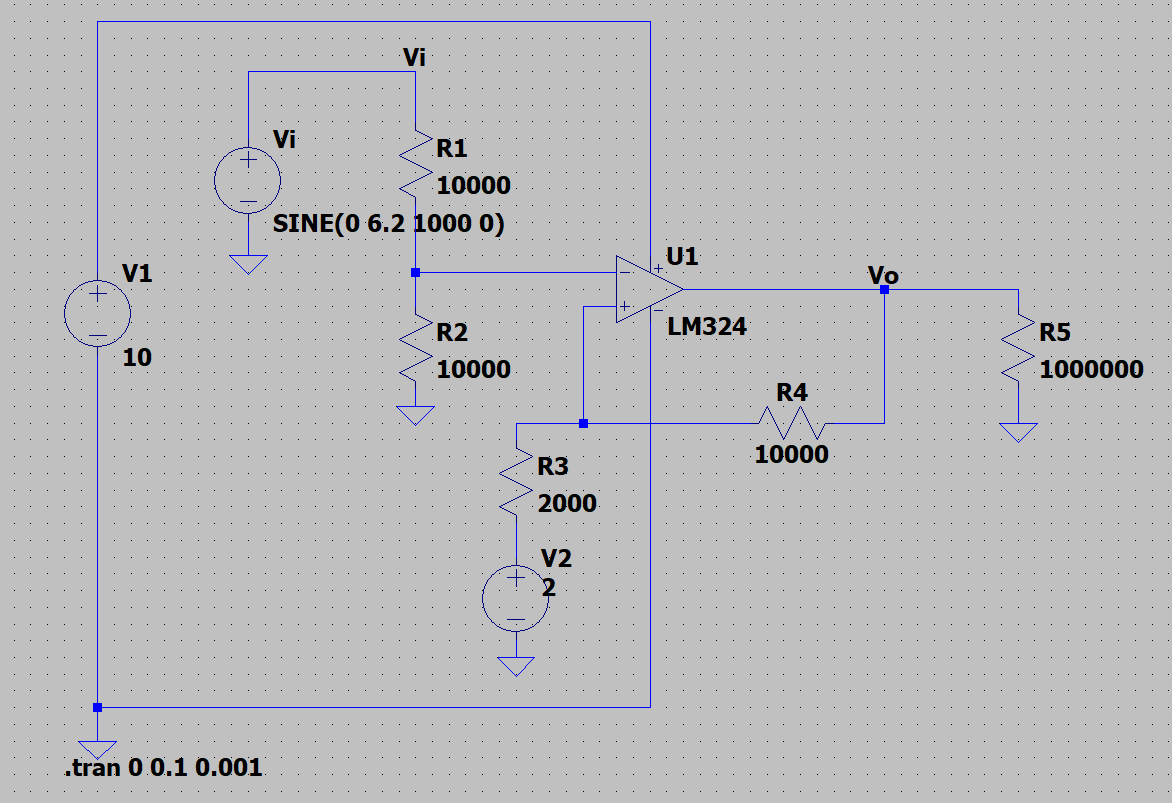
\includegraphics[width=1\linewidth]{Simulaciones-Resultados/Circuito4_esquematico}
		\caption{Comparador con histéresis}
		\label{fig:circuito4esquematico}
	\end{figure}
	Un comparador convencional simplemente compara dos voltajes de entrada y produce una salida alta o baja dependiendo de cuál sea mayor. Sin embargo, un comparador con histéresis introduce una especie de memoria en el circuito. Esto significa que una vez que la salida cambia de estado, se requiere un cambio más grande en la señal de entrada para que vuelva a cambiar. Esta característica es útil en muchas aplicaciones, como la detección de niveles, control de motores y circuitos de disparo.
	
	Analizamos por blackman y por superposición, cortamos por voltaje en la salida $V_{OUT}$ antes de $R4$, y arrancamos analizando $V_{OUT}$ con $V_{IN} = 0$ y $V_{REF} = 0$, obteniendo:
	\begin{equation}
		V_{o} = \frac{1}{6} A_{d} V'_{OUT}
	\end{equation}
	
	Luego hacemos $V_{OUT}$ para $V'_{OUT} = 0$ y $V_{REF} = 0$, y obtenemos:
	\begin{equation}
		V_{OUT} = -\frac{1}{2} A_{d} V_{IN}
	\end{equation}

	Por ultimo haremos $V_{OUT}$ para $V'_{IN} = 0$ y $V'_{OUT} = 0$, que nos da:
	\begin{equation}
		V_{OUT} = \frac{5}{6} A_{d} V_{REF}
	\end{equation}

	Si hacemos $V'_{OUT} = V_{OUT}$ y despejando obtenemos:

	\begin{equation}
		V_{OUT} = \frac{A_{d} \frac{1}{6} (5 V_{REF} - 3 V_{IN})}{1 - \frac{1}{6} A_{d}} = - (5 V_{REF} - 3V_{IN})
	\end{equation}
	
	\begin{figure}[]
		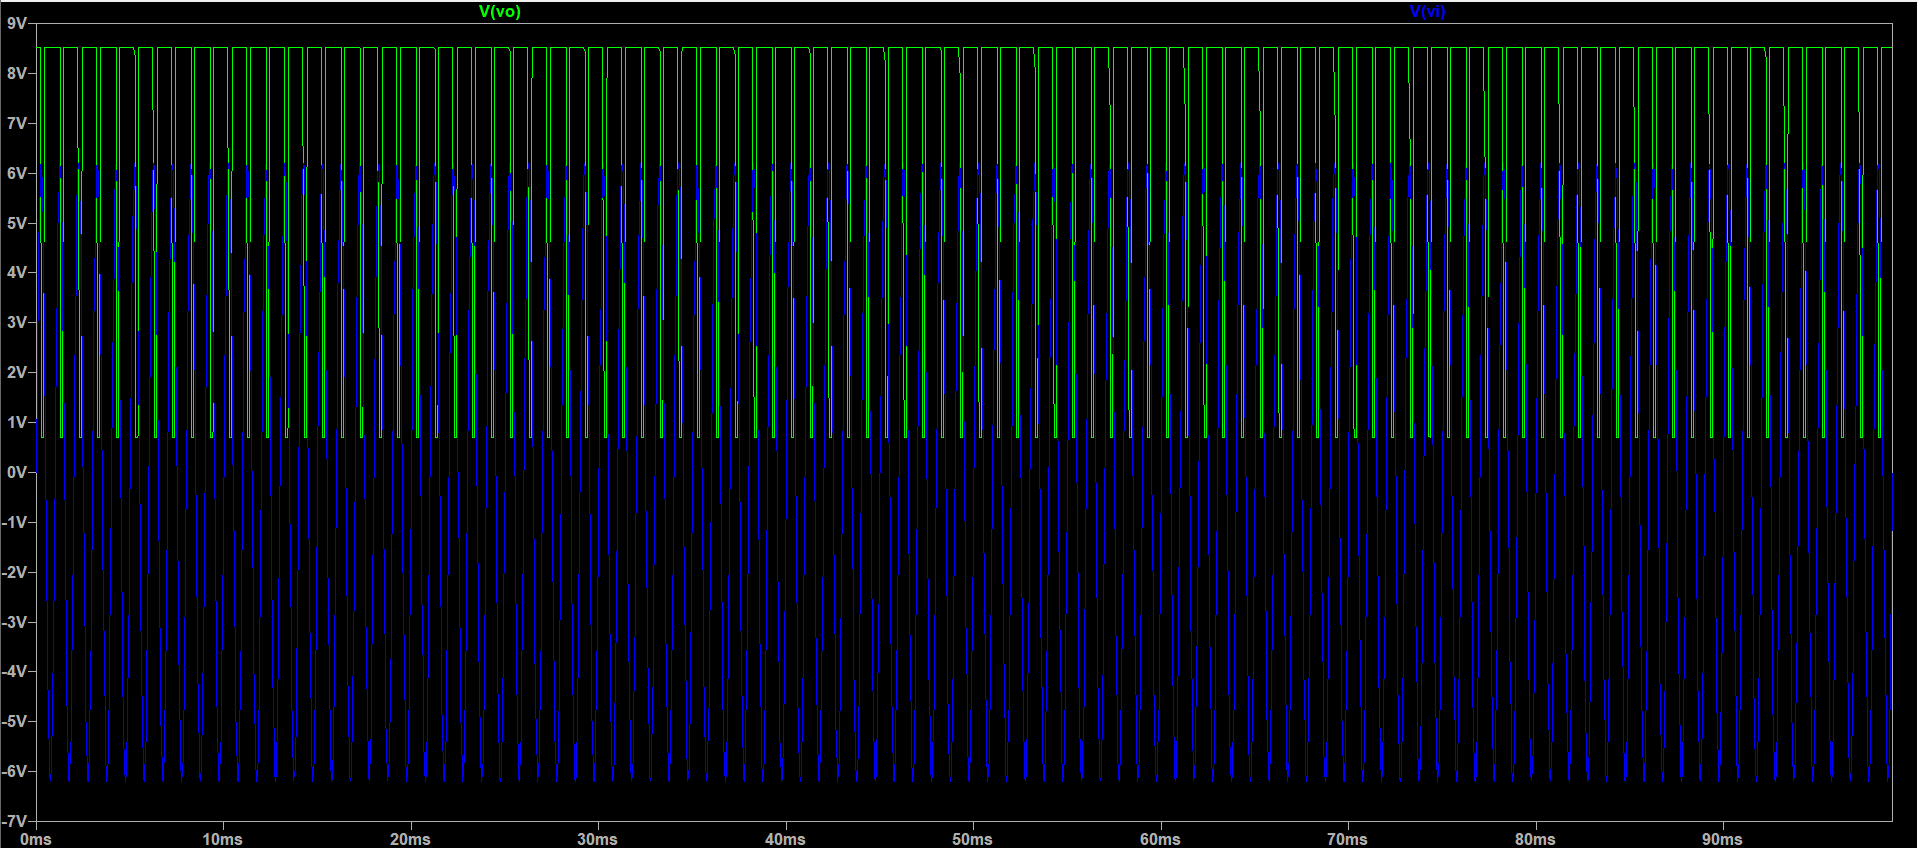
\includegraphics[width=1\linewidth]{Simulaciones-Resultados/Circuito4_Vo(Vi)}
		\caption[Salida del circuito]{Salida del circuito}
		\label{fig:circuito4vovi}
	\end{figure}
	En un amplificador operacional real, la impedancia de entrada es muy alta pero finita. En este circuito, la mayor parte de la corriente de entrada fluirá a través de $R1$ y $R2$. Por lo tanto, podemos aproximar la impedancia de entrada como la resistencia en paralelo de $R1$ y $R2$.
	
	\begin{equation}
		Z_{IN}=R1//R2=5[Kohm]
	\end{equation}


\end{document}
	}